
\documentclass[12pt]{article}
\topmargin=-1.0cm
\textheight=23cm
\evensidemargin=-1.0cm
\oddsidemargin=-1.0cm
\textwidth=19cm


\usepackage{pgfplots}
\pgfplotsset{width=10cm,compat=1.9}
% https://www.overleaf.com/learn/latex/Pgfplots_package#The_document_preamble

% TikZ - TikZ ist kein Zeichenprogramm:
\usepackage{tikz}
%\usetikzlibrary{calc}                 % maybe later
\usetikzlibrary{positioning}
\usetikzlibrary{arrows,intersections}

% PGF - Portable Graphics File:


% To define custom colors in plots - must appear after \usepackage{tikz}
\usepackage{color}
\definecolor{rsRed}   {rgb}{0.7,0.0,0.0}
\definecolor{rsYellow}{rgb}{0.5,0.4,0.0}
\definecolor{rsGreen} {rgb}{0.0,0.5,0.0}
\definecolor{rsCyan}  {rgb}{0.0,0.4,0.6}
\definecolor{rsBlue}  {rgb}{0.0,0.0,1.0}
\definecolor{rsPurple}{rgb}{0.5,0.0,0.8}

%\definecolor{mygray}{rgb}{0.5,0.5,0.5}
%\definecolor{mymauve}{rgb}{0.58,0,0.82}


\begin{document}

\title{Demo Plots with TikZ and PGF}
%\subtitle{(A Grab-Bag of Copy-And-Paste Recipes)}  % error!
\author{Robin Schmidt}
\maketitle

%===================================================================================================
\section{With TikZ}
Here, we show plots and graphics created with the TikZ package. This is a high level interface to PGF.

%---------------------------------------------------------------------------------------------------
\subsection{Monomials}
Figure \ref{Fig:Monomials} shows monomials of degrees up to 5 with \verb|xscale=6, yscale=3|. The even ones are drawn in red, the odd ones in blue.

\begin{figure}[h]
\centering
\caption{Monomials of degrees $0$ to $5$}
\label{Fig:Monomials}
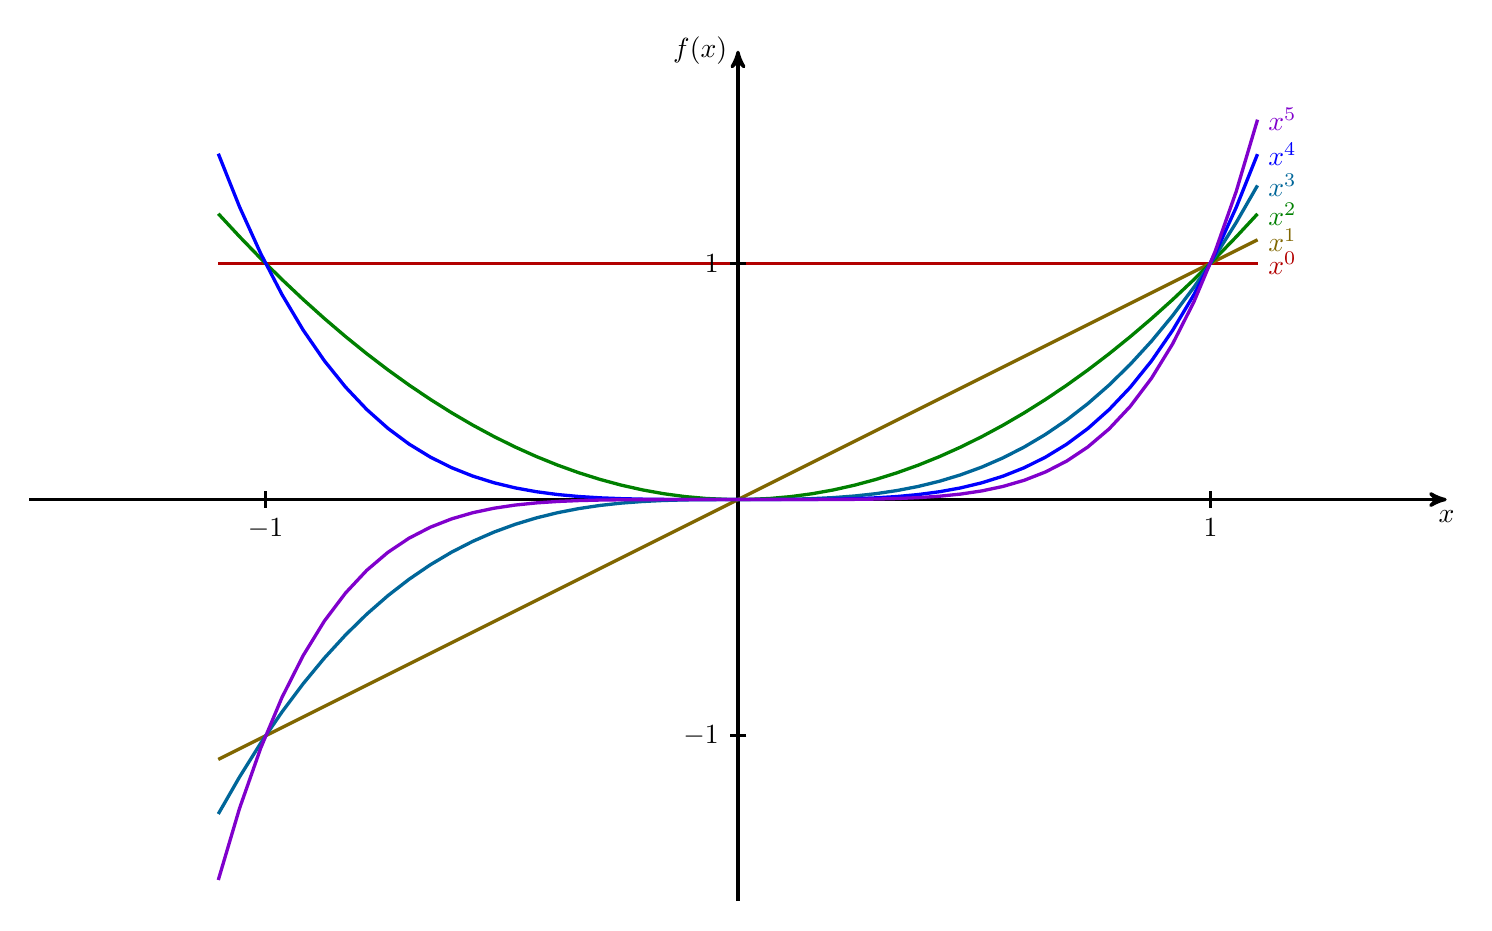
\begin{tikzpicture}
[domain=-1.1:1.1, range=-1.2:1.2, xscale=6, yscale=3, samples=50, very thick, >=stealth']

% Coordinate axes:
\draw[->] (-1.5,0) -- (1.5,0) node[below] {$x$};
\draw[->] (0,-1.7) -- (0,1.9) node[left]  {$f(x)$};

% Graphs:
\draw[color=rsRed]    plot (\x,{pow(\x,0)}) node[right] {$x^0$};
\draw[color=rsYellow] plot (\x,{pow(\x,1)}) node[right] {$x^1$};
\draw[color=rsGreen]  plot (\x,{pow(\x,2)}) node[right] {$x^2$};
\draw[color=rsCyan]   plot (\x,{pow(\x,3)}) node[right] {$x^3$};
\draw[color=rsBlue]   plot (\x,{pow(\x,4)}) node[right] {$x^4$};
\draw[color=rsPurple] plot (\x,{pow(\x,5)}) node[right] {$x^5$};

% Tick marks on x-axis:
\draw [shift={(-1,0)}] (0pt,+1pt) -- (0pt,-1pt) node [below] {$-1$};  
\draw [shift={( 1,0)}] (0pt,+1pt) -- (0pt,-1pt) node [below] {$1$};
% The point size 1pt results from 3 / yscale

% Tick marks on y-axis:
\draw [shift={(0,1)}]  (+.5pt, 0pt) -- (-.5pt, 0pt) node [left] {$1$};
\draw [shift={(0,-1)}] (+.5pt, 0pt) -- (-.5pt, 0pt) node [left] {$-1$};
% The point size .5pt results from 3 / xscale

\end{tikzpicture}
\end{figure}

%---------------------------------------------------------------------------------------------------
\subsection{Sine and Cosine}
Figure \ref{Fig:SineAndCosine} shows the sine and cosine function in default size, i.e. without using \verb|scale|, \verb|xscale|, \verb|yscale|. We draw the tick marks on the $x$-axis manually as short lines.

\begin{figure}[h]
\centering
\caption{Sine and cosine function}
\label{Fig:SineAndCosine}
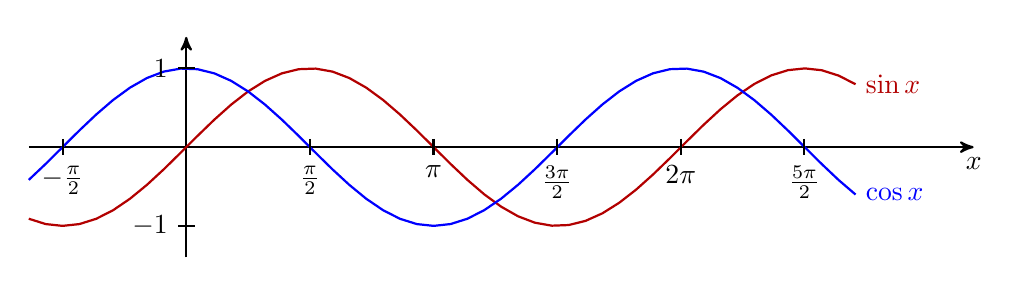
\begin{tikzpicture}
[domain=-2:8.5, samples=50, thick, >=stealth']

% Coordinate axes:
\draw[->] (-2.0,0) -- (10.0,0) node[below] {$x$};
\draw[->] (0,-1.4) -- (0,1.4) node[left]  {};

% Graphs of sin(x) and cos(x):
\draw[color=rsRed]   plot (\x,{sin(\x r)}) node[right] {$\sin x$};
\draw[color=rsBlue]  plot (\x,{cos(\x r)}) node[right] {$\cos x$};
% \x r means to convert '\x' from degrees to radians
  
% Tick marks on x-axis:
\draw [shift={(-1.57,0)}] (0pt,+3pt) -- (0pt,-3pt) node [below] {$-\frac{\pi}{2}$};  
\draw [shift={( 1.57,0)}] (0pt,+3pt) -- (0pt,-3pt) node [below] {$\frac{\pi}{2}$};
\draw [shift={( 3.14,0)}] (0pt,+3pt) -- (0pt,-3pt) node [below] {$\pi$};
\draw [shift={( 4.71,0)}] (0pt,+3pt) -- (0pt,-3pt) node [below] {$\frac{3\pi}{2}$};
\draw [shift={( 6.28,0)}] (0pt,+3pt) -- (0pt,-3pt) node [below] {$2\pi$};
\draw [shift={( 7.85,0)}] (0pt,+3pt) -- (0pt,-3pt) node [below] {$\frac{5\pi}{2}$};  
  
% Tick marks on y-axis:
\draw [shift={(0,1)}]  (+3pt, 0pt) -- (-3pt, 0pt) node [left] {$1$};
\draw [shift={(0,-1)}] (+3pt, 0pt) -- (-3pt, 0pt) node [left] {$-1$};
    
\end{tikzpicture}
\end{figure}


%---------------------------------------------------------------------------------------------------
\subsection{Line Equations}
Figure \ref{Fig:Line} shows a line defined by two points $\mathbf{p}_1, \mathbf{p}_2$ and various forms of the line equation embedded in the plot. It also shows how to draw dots and arrows and a coordinate grid. There's also an angle $\alpha$ drawn by a circular arc.

\begin{figure}[h]
\centering
\caption{Line Equations}
\label{Fig:Line}
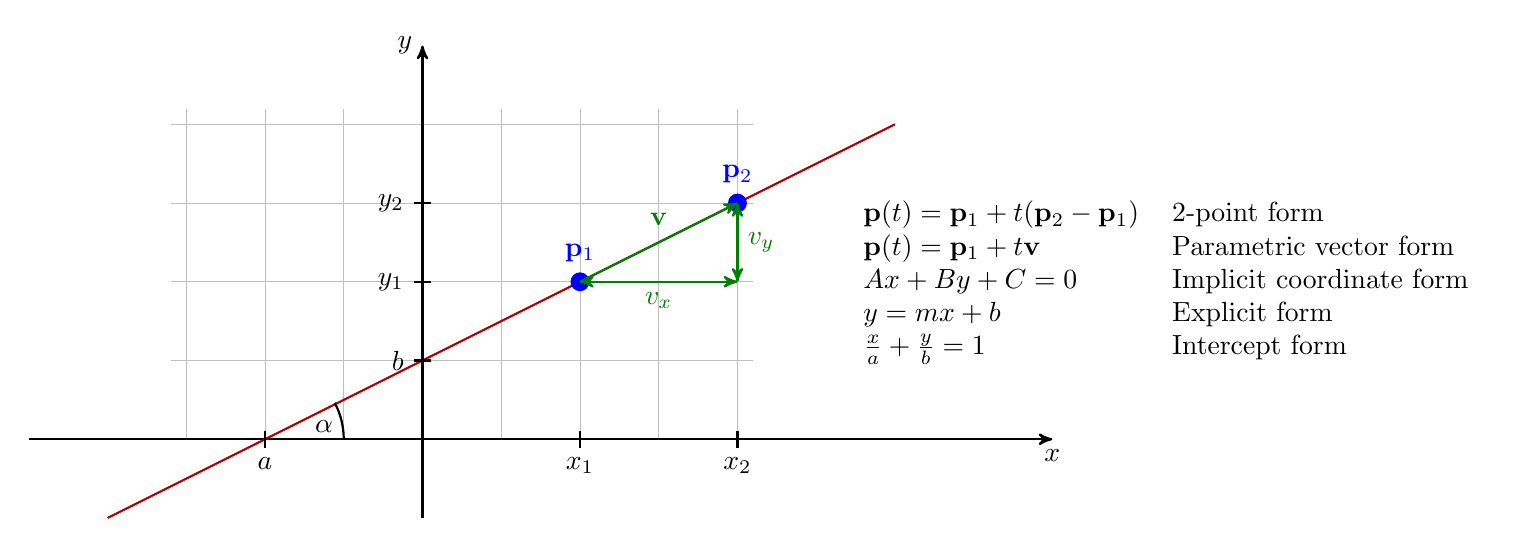
\begin{tikzpicture}
[thick, >=stealth', 
  dot/.style = { draw, fill = black, circle, inner sep = 0pt, minimum size = 6pt }
]

% Grid:
\draw[very thin,color=lightgray] (-3.2,0.0) grid (4.2,4.2);

% Coordinate system:
\draw[->] (-5, 0) -- (8,0) coordinate[label = {below:$x$}] (xmax);
\draw[->] ( 0,-1) -- (0,5) coordinate[label = {left:$y$}]  (ymax);

% Line:  
\draw[rsRed]     (-4,-1) -- (6,4)  node[pos=0.85, below right] {};

% Points 1p, p2 on the line:  
\draw[rsBlue] (2,2) node[dot, rsBlue, label = {above:$\mathbf{p}_1$}]{};
\draw[rsBlue] (4,3) node[dot, rsBlue, label = {above:$\mathbf{p}_2$}]{};
% When using rsBlue only inside the node, only the dot becomes blue

% Vector v and its components:
\draw[rsGreen, <->] (2,2) -- (4,2);
\draw[rsGreen] (3,2) node[below] {$v_x$};
\draw[rsGreen, <->] (4,2) -- (4,3);
\draw[rsGreen] (4,2.5) node[right] {$v_y$};
\draw[rsGreen, ->] (2,2) -- (4,3);
\draw[rsGreen] (3,3) node[below] {$\mathbf{v}$};

% Marks on the x- and y-axes:
% ToDo: try to use tick-marks instead - or just drop horizontal and vertical lines
% Maybe draw a grid
\draw [shift={(2,0)}, color=black] ( 0pt,+3pt) -- ( 0pt,-3pt) node [below] {$x_1$};
\draw [shift={(4,0)}, color=black] ( 0pt,+3pt) -- ( 0pt,-3pt) node [below] {$x_2$};
\draw [shift={(0,2)}, color=black] (+3pt, 0pt) -- (-3pt, 0pt) node [left]  {$y_1$};
\draw [shift={(0,3)}, color=black] (+3pt, 0pt) -- (-3pt, 0pt) node [left]  {$y_2$};

% x,y intercepts:
\draw [shift={(-2,0)}, color=black] ( 0pt,+3pt) -- ( 0pt,-3pt) node [below] {$a$};
\draw [shift={( 0,1)}, color=black] (+3pt, 0pt) -- (-3pt, 0pt) node [left]  {$b$};

% angle alpha:
\draw (-1,0) arc (0:27.5:1);
\draw (-1.25,0.16) node[label = {center:$\alpha$}]{};

% Equations:
\node[align=left] at (9.5,2.0) 
{
\begin{tabular}{l l}
  $\mathbf{p}(t) = \mathbf{p}_1 + t (\mathbf{p}_2 -\mathbf{p}_1)$ & 2-point form \\
  $\mathbf{p}(t) = \mathbf{p}_1 + t \mathbf{v}$ & Parametric vector form \\  
  $Ax + By + C = 0$                             & Implicit coordinate form \\   
  $y = m x + b$                                 & Explicit form \\
  $\frac{x}{a} + \frac{y}{b} = 1$               & Intercept form \\
\end{tabular}
};
\end{tikzpicture}
\end{figure}

%---------------------------------------------------------------------------------------------------
\subsection{Riemann Integral}

\newcommand\ra{-1} % ra = Riemann, a
\newcommand\ratwo{-0.5} % ra = Riemann, a
\newcommand\rb{4} % rb = Riemann, b
\newcommand\rbtwo{3.5} % rb = Riemann, b

\textcolor{blue}{Left-hand Riemann Sum} and 
\textcolor{red}{Right-hand Riemann Sum}

\begin{tikzpicture}

    \draw[<->] (\ra-0.5,0) -- (\rb+0.5,0);
    \draw[<->] (0,\ra-0.5) -- (0,\rb+0.5);
    \draw[dashed] (\ra,0) -- (\ra,1) node[above] {$a$};
    \draw[dashed] (\rb,0) -- (\rb,-1) node[below] {$b$};
    
    %Right-Hand
    \foreach \x in {\ratwo,0,...,\rb} % <--- my issues
    \draw[thick, fill=red!25] (\x-.5,0) -- (\x-.5,{sin(deg(\x))}) -- (\x,{sin(deg(\x))}) -- (\x,0) -- cycle;
    
    %Left-Hand
    \foreach \x in {\ra,-0.5,...,\rbtwo} % <--- my issues
    \draw[thick, fill=blue!25] (\x,0) -- (\x,{sin(deg(\x))}) -- (\x+.5,{sin(deg(\x))}) -- (\x+.5,0) -- cycle;
    
    \draw[ultra thick, <->, domain=\ra:\rb, smooth, samples=100, variable=\x] plot ({\x},{sin(deg(\x))});
    
\end{tikzpicture}

%\begin{figure}[h]
%\centering
%\caption{Line Equations}
%\label{Fig:RiemannIntegral}
%\end{figure}

% ToDo: triangles, polygons, ...

% https://tex.stackexchange.com/questions/554044/riemann-integral-on-tikz-with-commands

%===================================================================================================
\section{With PGFPlots}

%---------------------------------------------------------------------------------------------------
\subsection{Taylor Polynomials}
The figures \ref{Fig:TaylorExpansionSine}, \ref{Fig:TaylorExpansionCosine}, \ref{Fig:TaylorExpansionExp} show the first couple of Taylor polynomials for $\sin, \cos, \exp$ respectively.

\pgfplotsset{width=19cm,height=6cm,compat=1.9}

\begin{figure}[h]
\centering
\caption{Sine function and its Taylor polynomials}
\label{Fig:TaylorExpansionSine}
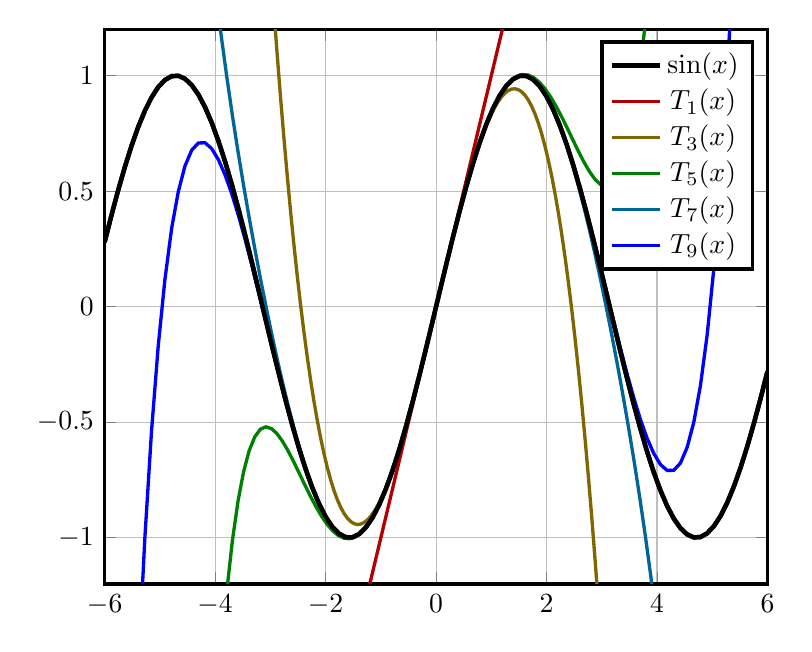
\begin{tikzpicture}
\begin{axis}[xmin=-6, xmax=6, ymin=-1.2, ymax=1.2, samples=100, very thick, 
             xmajorgrids=true, ymajorgrids=true]

  \addplot[domain=-6:6, color=black, ultra thick] {sin( \x r )};
  \addlegendentry{\(\sin(x)\)}
  
  \addplot[domain=-6:6, color=rsRed] {x};
  \addlegendentry{$T_1(x)$}
  
 \addplot[domain=-3:3, color=rsYellow] {\x - \x^3/6};
  \addlegendentry{$T_3(x)$}
  
 \addplot[domain=-5:5, color=rsGreen] {\x - \x^3/6 + \x^5/120};
 \addlegendentry{$T_5(x)$}
  
 \addplot[domain=-5:5, color=rsCyan] {\x - \x^3/6 + \x^5/120 - \x^7/5040};
 \addlegendentry{$T_7(x)$}
  
 \addplot[domain=-6:6, color=rsBlue] {\x - \x^3/6 + \x^5/120 - \x^7/5040 + \x^9/362880};
 \addlegendentry{$T_9(x)$}
 
 \addplot[domain=-6:6, color=black, ultra thick] {sin( \x r )}; 
 
\end{axis}
\end{tikzpicture}
\end{figure}


\begin{figure}[h]
\centering
\caption{Cosine function and its Taylor polynomials}
\label{Fig:TaylorExpansionCosine}
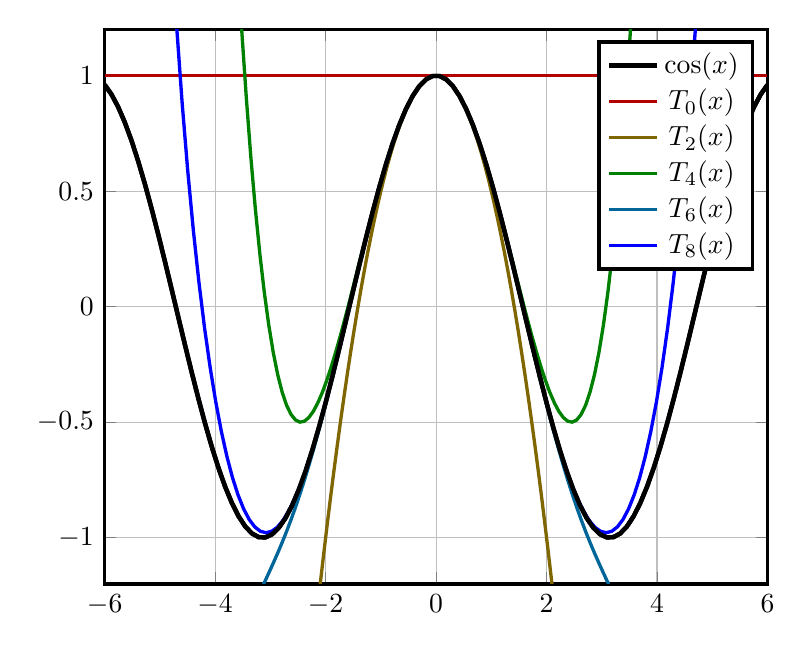
\begin{tikzpicture}
\begin{axis}[xmin=-6, xmax=6, ymin=-1.2, ymax=1.2, samples=100, very thick, 
             xmajorgrids=true, ymajorgrids=true]

  \addplot[domain=-6:6, color=black, ultra thick] {cos( \x r )};
  \addlegendentry{\(\cos(x)\)}
  
  \addplot[domain=-6:6, color=rsRed] {1};
  \addlegendentry{$T_0(x)$}
  
  \addplot[domain=-3:3, color=rsYellow] {1 - \x^2/2};
  \addlegendentry{$T_2(x)$}
  
  \addplot[domain=-4:4, color=rsGreen] {1 - \x^2/2 + \x^4/24};
  \addlegendentry{$T_4(x)$}
  
  \addplot[domain=-4:4, color=rsCyan] {1 - \x^2/2 + \x^4/24 - \x^6/720};
  \addlegendentry{$T_6(x)$}  
  
  \addplot[domain=-5:5, color=rsBlue] {1 - \x^2/2 + \x^4/24 - \x^6/720 + \x^8/40320};
  \addlegendentry{$T_8(x)$} 

  \addplot[domain=-6:6, color=black, ultra thick] {cos( \x r )};

\end{axis}
\end{tikzpicture}
\end{figure}


\pgfplotsset{width=15cm,height=10cm,compat=1.9}

\begin{figure}[h]
\centering
\caption{Exponential function and its Taylor polynomials}
\label{Fig:TaylorExpansionExp}
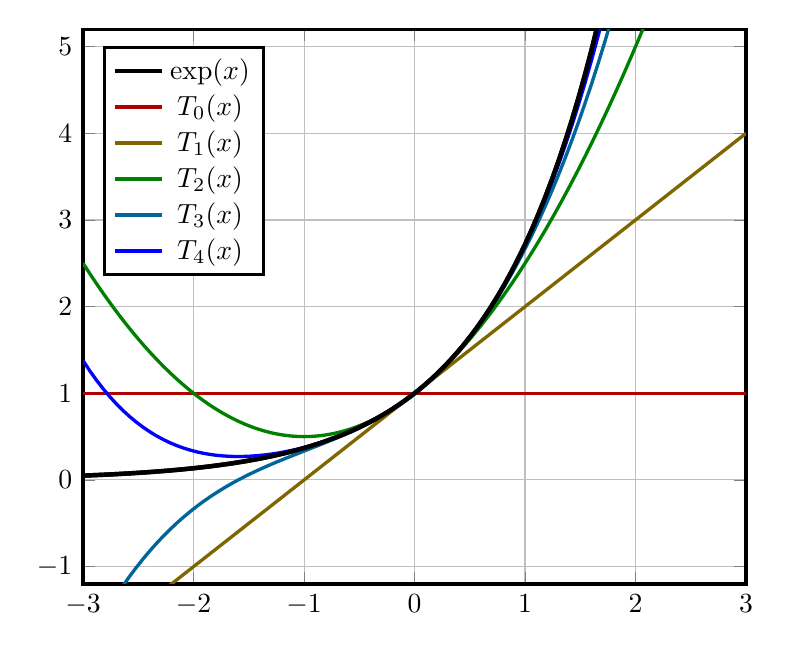
\begin{tikzpicture}
\begin{axis}[xmin=-3, xmax=3, ymin=-1.2, ymax=5.2, samples=100, very thick, 
             legend pos=north west, xmajorgrids=true, ymajorgrids=true]

  \addplot[domain=-3:3, color=black, ultra thick] {exp(\x )};
  \addlegendentry{$\exp(x)$}
  
  \addplot[domain=-3:3, color=rsRed] {1};
  \addlegendentry{$T_0(x)$}
  
  \addplot[domain=-3:3, color=rsYellow] {1 + x};
  \addlegendentry{$T_1(x)$}  
  
  \addplot[domain=-3:3, color=rsGreen] {1 + x + x^2/2};
  \addlegendentry{$T_2(x)$}    
  
  \addplot[domain=-3:3, color=rsCyan] {1 + x + x^2/2 + x^3/6};
  \addlegendentry{$T_3(x)$}
  
  \addplot[domain=-3:3, color=rsBlue] {1 + x + x^2/2 + x^3/6 + x^4/24};
  \addlegendentry{$T_4(x)$}  
  
  % draw the exp again so it is in the foreground:
  \addplot[domain=-3:3, color=black, ultra thick] {exp(\x )};
  
\end{axis}
\end{tikzpicture}
\end{figure}



% ToDo: 1 / (1 + x^2), 1 / (1 - x^2)

% plots for:
% -Fourier polynomials
% -Derivative
% -Riemann integral, Lebesgue integral

%---------------------------------------------------------------------------------------------------
\subsection{Bivariate Functions}
To plot bivariate functions, one can use the command \verb|\addplot3|. It can be configured to to do surface plots or heat maps. This is shown in figures \ref{Fig:BivariateGaussian3D} and \ref{Fig:BivariateGaussianHeatMap}. 

%\pgfplotsset{width=12cm,height=8cm,compat=1.9}
\pgfplotsset{width=16cm,height=10cm,compat=1.9}

\begin{figure}[h]
\centering
\caption{$f(x,y) = x e^{-(x^2+y^2)}$}
\label{Fig:BivariateGaussian3D}
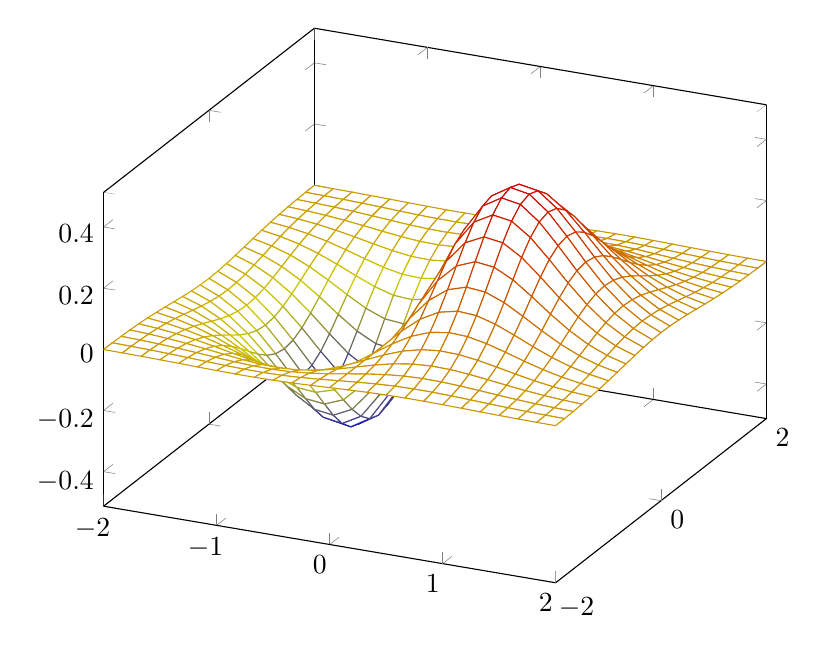
\begin{tikzpicture}
\begin{axis}
   %[title=Bivariate Gaussian]
   \addplot3 [surf,fill=white,domain=-2:2] {x * exp(-x^2-y^2)};
\end{axis}
\end{tikzpicture}
\end{figure}


%\pgfplotsset{width=12cm,height=8cm,compat=1.9}

\begin{figure}[h]
\centering
\caption{$f(x,y) = x e^{-(x^2+y^2)}$}
\label{Fig:BivariateGaussianHeatMap}
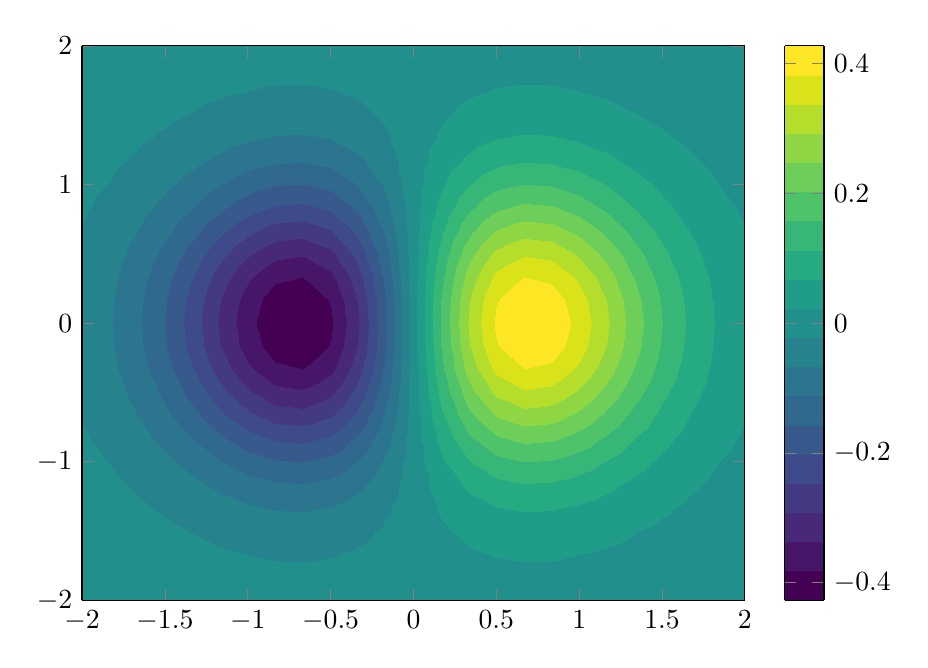
\begin{tikzpicture}
\begin{axis}[
%    title={$x \exp(-x^2-y^2)$},
    domain=-2:2, view={0}{90}, colorbar right, colormap name = viridis ]
    
  \addplot3 [contour filled={number=19,},] 
  {exp(-x^2-y^2)*x};
  
\end{axis}
\end{tikzpicture}
\end{figure}


% colormaps: viridis

% https://tikz.dev/pgfplots/reference-3dplots

% https://stackoverflow.com/questions/70338079/get-east-position-of-tikz-legend
% Has example for loading data from .csv file

% Line thickness options: semithick, thick, very thick, ultra thick, line width=4pt

% plotting data from files:
% https://tikz.dev/pgfplots/reference-addplot#sec-4.3.4
% \addplot table {filename.txt}

%===================================================================================================
%\section{With Both}



\end{document}